\documentclass[12pt]{beamer}
\usetheme{default}
\usepackage[labelformat=empty]{subfig}

\usepackage{amsfonts}
\usepackage{stmaryrd}
\usepackage{upgreek}
\usepackage{url}


\usepackage[greek,english]{babel}


\DeclareMathAlphabet{\mathkw}{OT1}{cmss}{bx}{n}

\usepackage{color}
\newcommand{\redFG}[1]{\textcolor[rgb]{0.6,0,0}{#1}}
\newcommand{\greenFG}[1]{\textcolor[rgb]{0,0.4,0}{#1}}
\newcommand{\blueFG}[1]{\textcolor[rgb]{0,0,0.8}{#1}}
\newcommand{\orangeFG}[1]{\textcolor[rgb]{0.8,0.4,0}{#1}}
\newcommand{\purpleFG}[1]{\textcolor[rgb]{0.4,0,0.4}{#1}}
\newcommand{\yellowFG}[1]{\textcolor{yellow}{#1}}
\newcommand{\brownFG}[1]{\textcolor[rgb]{0.5,0.2,0.2}{#1}}
\newcommand{\blackFG}[1]{\textcolor[rgb]{0,0,0}{#1}}
\newcommand{\whiteFG}[1]{\textcolor[rgb]{1,1,1}{#1}}
\newcommand{\yellowBG}[1]{\colorbox[rgb]{1,1,0.2}{#1}}
\newcommand{\brownBG}[1]{\colorbox[rgb]{1.0,0.7,0.4}{#1}}

\newcommand{\ColourStuff}{
  \newcommand{\red}{\redFG}
  \newcommand{\green}{\greenFG}
  \newcommand{\blue}{\blueFG}
  \newcommand{\orange}{\orangeFG}
  \newcommand{\purple}{\purpleFG}
  \newcommand{\yellow}{\yellowFG}
  \newcommand{\brown}{\brownFG}
  \newcommand{\black}{\blackFG}
  \newcommand{\white}{\whiteFG}
}

\newcommand{\MonochromeStuff}{
  \newcommand{\red}{\blackFG}
  \newcommand{\green}{\blackFG}
  \newcommand{\blue}{\blackFG}
  \newcommand{\orange}{\blackFG}
  \newcommand{\purple}{\blackFG}
  \newcommand{\yellow}{\blackFG}
  \newcommand{\brown}{\blackFG}
  \newcommand{\black}{\blackFG}
  \newcommand{\white}{\blackFG}
}

\ColourStuff

\newcommand{\K}[1]{\yellow{\mathsf{#1}}}
\newcommand{\I}[1]{\green{\mathsf{#1}}}
\newcommand{\D}[1]{\blue{\mathsf{#1}}}
\newcommand{\C}[1]{\red{\mathsf{#1}}}
\newcommand{\F}[1]{\green{\mathsf{#1}}}
\newcommand{\V}[1]{\purple{\mathit{#1}}}

\usepackage{ucs}
\usepackage[utf8x]{inputenc}

%include lhs2TeX.fmt
%include lhs2TeX.sty
%include polycode.fmt

\DeclareUnicodeCharacter{949}{\varepsilon} % ε
\DeclareUnicodeCharacter{8702}{QQQQQQQQQQQQQQQQQQ} % QQQ
\DeclareUnicodeCharacter{737}{^{l}} % ˡ
\DeclareUnicodeCharacter{8759}{\colon\colon} % ∷

\newcommand{\seq}{\gg}
\newcommand{\hyp}{\text{-}}

%format Set = "\I{Set}"
%format List = "\I{List}"
%format × = "\I{×}"
%format ⊎ = "\I{⊎}"
%format ∘ = "\I{∘}"
%format map = "\I{map}"
%format flip = "\I{flip}"
%format foldr = "\I{foldr}"


%format + = "\D{+}"
%format _+_ = "\_" + "\_"
%format ⇾ = "\D{\seq}"
%format _⇾_ = "\_" ⇾ "\_"
%format ⇾-assoc ="\D{\seq{}assoc}"
%format +-assoc ="\D{+assoc}"
%format +-comm = "\D{+comm}"
%format ⇾-identityˡ = "\D{\seq{}identity^l}"
%format ⇾-identityʳ = "\D{\seq{}identity^r}"
%format distribʳ = "\D{distrib^r}"
%format distribˡ = "\D{distrib^l}"
%format decomposition = "\D{decomposition}"
%format ⇾ʳ = "\D{\seq{}_r}"
%format ⇾₁ = "\D{\seq{}_1}"
%format _⇾₁_ = "\_" ⇾₁ "\_"
%format _⇾ʳ_ = "\_" ⇾ʳ "\_"
%format ∷ = "\C{::}"
%format ε = "\D{\varepsilon}"
%format G = "\D{G}"
%format B = "\D{B}"
%format ≈ = "\D{≈}"
%format _≈_ = "\_" ≈ "\_"

\title{Machine-assisted Formalisation of Parametrised Graph Algebra}

\author[A. Alekseyev, A. Mokhov, A. Yakovlev, A. Bystrov]{Arseniy Alekseyev, Andrey Mokhov, \\ Alex Yakovlev, Alex Bystrov}

\institute[EECE MSD]{
  Microelectronic System Design Group \\
  Department of EECE \\
  Newcastle University
}

\date{January 26, 2012}

\begin{document}

\begin{frame}
  \titlepage
\end{frame}

\begin{frame}{Describing hardware microcontrollers}

Low level options:

\begin{itemize}
  \item Logic gate circuits
  \item State machines
  \item ...
\end{itemize}

High level options:

\begin{itemize}
  \item Petri nets
  \item Process algebra
  \item High-level languages
  \item ...
\end{itemize}

\end{frame}

\begin{frame}{Conditional Partial Order Graphs}
\begin{itemize}
\item Vertices represent events
\item Edges represent causal dependencies
\item Annotated with conditions
\end{itemize}

\begin{centering}
\hfill{}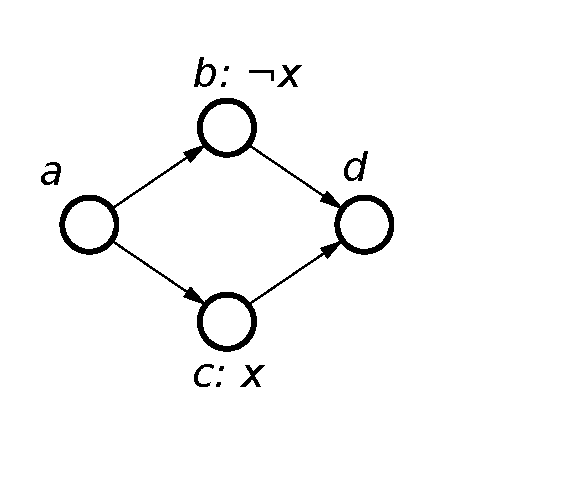
\includegraphics[scale=0.5]{fig/cpog_example}\hfill{}
\end{centering}

\end{frame}

\begin{frame}{Parametrised Graph Algebra}
PG Algebra is a generalisation of CPOGs

\begin{itemize}
\item Arbitrary set together with algebraic operations on it
\item Equivalence relation satisfying certain laws
\end{itemize}

\begin{figure}[h]
\begin{centering}
\hfill{}\subfloat[$G_{1} = a \seq b + c$]{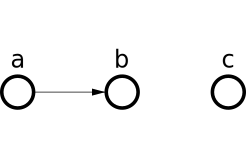
\includegraphics[scale=0.35]{fig/graph_3}
}\hfill{}\hfill{}\subfloat[$G_{2} = d$]{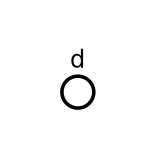
\includegraphics[scale=0.35]{fig/graph_4}
}\hfill{}\hfill{}\subfloat[$G_{1}+G_{2}$]{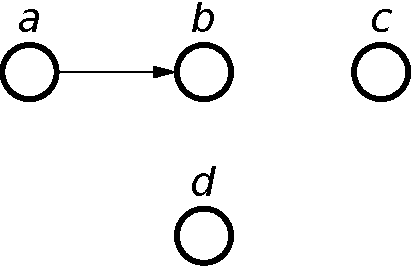
\includegraphics[scale=0.35]{fig/graph_overlay_3_4}
}\hfill{}\hfill{}\subfloat[$G_{1}\seq G_{2}$]{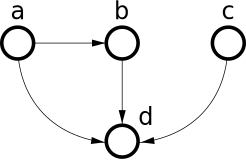
\includegraphics[scale=0.35]{fig/graph_sequence_3_4}
}\hfill{}
\par\end{centering}
\end{figure}
\end{frame}

\begin{frame}{Desired PG software support}
\begin{itemize}
\item Formula manipulations
\item Conversions to/from different formalisms
\item Hardware synthesis
\end{itemize}
\end{frame}
\begin{frame}{Formal methods}
\begin{itemize}
\item How do we know the theory is sound?
\item How do we know the tools are correct?
\item Need a way to statically ensure this.
\end{itemize}
\end{frame}
\begin{frame}{Agda}
Why Agda?
\begin{itemize}
\item A total functional programming language
\item A proof environment based on Curry-Howard isomorphism
\item Easy to learn when you know Haskell
\item Newbie-friendly community
\end{itemize}
\end{frame}

\begin{frame}{Graph Algebra}

%format cond0 = "\D{[}\_\D{]}\_"
%format GraphOps = "\D{GraphOps}"
%format IsGraphAlgebra = "\D{IsGraphAlgebra}"

\small{

\begin{code}
record GraphOps G : Set where
 field
  ε : G
  _+_ : G → G → G
  _⇾_ : G → G → G

record IsGraphAlgebra : Set where
 field
  +-assoc       : ∀ {p q r} → (p + q) + r ≈ p + (q + r)
  +-comm        : ∀ {p q}   → p + q ≈ q + p
  ⇾-assoc       : ∀ {p q r} → (p ⇾ q) ⇾ r ≈ p ⇾ (q ⇾ r)
  ⇾-identityˡ   : ∀ {p}     → ε ⇾ p ≈ p
  ⇾-identityʳ   : ∀ {p}     → p ⇾ ε ≈ p
  distribˡ      : ∀ {p q r} → p ⇾ (q + r) ≈ p ⇾ q + p ⇾ r
  distribʳ      : ∀ {p q r} → (p + q) ⇾ r ≈ p ⇾ r + q ⇾ r
  decomposition : ∀ {p q r} → p ⇾ q ⇾ r ≈ p ⇾ q + p ⇾ r + q ⇾ r
\end{code}
}
\end{frame}

\begin{frame}{Introducing conditions}
\begin{code}
  cond0 : B → G → G
\end{code}

%format true-condition = "\D{true\hyp{}condition}"
%format false-condition = "\D{false\hyp{}condition}"
%format and-condition = "\D{and\hyp{}condition}"
%format or-condition = "\D{or\hyp{}condition}"
%format conditional-+ = "\D{conditional+}"
%format conditional-⇾ = "\D{conditional\!\seq}"
%format boolean-algebra = "\D{boolean\hyp{}algebra}"
%format BooleanAlgebra = "\D{BooleanAlgebra}"

%format +-identity = "\D{+identity}"
%format +-idempotence = "\D{+idempotence}"
%format absorptionʳ = "\D{absorption^r}"
%format absorptionˡ = "\D{absorption^l}"

%format ∧ = "\D{∧}"
%format _∧_ = "\_" ∧ "\_"
%format ∨ = "\D{∨}"
%format _∨_ = "\_" ∨ "\_"
%format ¬_ = ¬ "\_"
%format ¬ = "\D{¬}"
%format ⊤ = "\D{⊤}"
%format ⊥ = "\D{⊥}"

%format [ = "\D{[}"
%format ] = "\D{]}"

%format choice-propagation₁ = "\D{choice\hyp{}propagation_1}"
%format choice-propagation₂ = "\D{choice\hyp{}propagation_2}"
%format condition-regularisation = "\D{condition\hyp{}regularisation}"


\begin{code}
  boolean-algebra : BooleanAlgebra B
  true-condition : ∀ x → [ ⊤ ] x ≈ x
  false-condition : ∀ x → [ ⊥ ] x ≈ ε
  and-condition : ∀ f g x → [ f ∧ g ] x ≈ [ f ] [ g ]  x
  or-condition : ∀ f g x → [ f ∨ g ] x ≈ [ f ] x + [ g ]  x
  conditional-+ : ∀ f x y → [ f ] (x + y) ≈ [ f ] x + [ f ] y
  conditional-⇾ : ∀ f x y → [ f ] (x ⇾ y) ≈ [ f ] x ⇾ [ f ] y
\end{code}
\end{frame}

\begin{frame}{PG Algebra theorems}

The following theorems has been derived from the axioms:

\begin{code}
+-identity : ∀ p → p + ε ≈ p

+-idempotence : ∀ p → p + p ≈ p

absorptionˡ : ∀ p q → p ⇾ q + p ≈ p ⇾ q

absorptionʳ : ∀ p q → p ⇾ q + q ≈ p ⇾ q

choice-propagation₁ : ∀ b p q r → 
  [ b ] (p ⇾ q) + [ ¬ b ] (p ⇾ r) ≈ p ⇾ ([ b ] q + [ ¬ b ] r) 

choice-propagation₂ : ∀ b p q r → 
  [ b ] (p ⇾ r) + [ ¬ b ] (q ⇾ r) ≈ ([ b ] p + [ ¬ b ] q) ⇾ r

condition-regularisation : ∀ f g p q → 
  [ f ] p ⇾ [ g ] q ≈ [ f ] p + [ g ] q + [ f ∧ g ] (p ⇾ q)
\end{code}
\end{frame}

%format A = "\D{A}"
%format PGFormula = "\D{PGFormula}"

%format + = "\C{+}"
%format _+_ = "\_" + "\_"
%format ⇾ = "\C{\seq}"
%format _⇾_ = "\_" ⇾ "\_"
%format ε = "\C{ε}"
%format var = "\C{var}"
%format cond0 = "\C{[}\_\C{]}\_"
%format [ = "\C{[}"
%format ] = "\C{]}"

%format _+-s_ = "\_\D{+_s}\_"
%format _⇾-s_ = "\_\D{\seq_s}\_"
%format ε-s = "\D{ε_s}"
%format cond-s = "\D{[}\_\D{]_s}\_"
%format var-s = "\D{var_s}"

%format BoolFormula = "\D{BoolFormula}"

%format ∧ = "\C{∧}"
%format _∧_ = "\_" ∧ "\_"
%format ∨ = "\C{∨}"
%format _∨_ = "\_" ∨ "\_"
%format ¬_ = ¬ "\_"
%format ¬ = "\C{¬}"
%format ⊤ = "\C{⊤}"
%format ⊥ = "\C{⊥}"

%format ⇾-assoc ="\C{\seq{}assoc}"
%format +-assoc ="\C{+assoc}"
%format +-comm = "\C{+comm}"
%format V = "\D{V}"

%format BF = "\D{BF}"
%format PG = "\D{PG}"
%format NF = "\D{NF}"
%format Lit = "\D{Lit}"
%format Node = "\D{Node}"


%format inj₁ = "\C{inj_1}"
%format inj₂ = "\C{inj_2}"
%format fromNode = "\D{fromNode}"
%format , = "\C{,}"
%format mkt = "\_\C{,}\_"
%format fromLit = "\D{fromLit}"
%format fromNF = "\D{fromNF}"
%format +-nf = "\D{+_{NF}}"
%format ⇾-nf = "\D{\seq_{NF}}"
%format _⇾-nf_ = "\_" ⇾-nf "\_"
%format _+-nf_ = "\_" +-nf "\_"
%format fromVar = "\D{fromVar}"
%format addCondition = "\D{addCondition}"
%format normalise = "\D{normalise}"

%format normalise-correct = "\D{normalise\hyp{}correct}"


%format pg-eval = "\D{pg\hyp{}eval}"
%format ≈f = "\D{≈_{f}}"
%format _≈f_ = "\_" ≈f "\_"


\begin{frame}{Formula data structure}

Formula data structure mimics the algebra operations:

\begin{code}
 data PGFormula B V : Set where
  _+_ : (x y : PGFormula) → PGFormula
  _⇾_ : (x y : PGFormula) → PGFormula
  ε : PGFormula
  var : (a : V) → PGFormula
  [_]_ : (c : B) → PGFormula → PGFormula
\end{code}
\end{frame}

\begin{frame}{Making sense of the formulae}

We need to give the formula semantics in terms of algebra.

\begin{code}
pg-eval : PGFormula B V
    → (V → G) 
    → PGAlgebra G V
    → G
\end{code}
\begin{code}
_≈f_ : PGFormula B V → PGFormula B V → Set
a ≈f b = ∀ assign alg 
         → pg-eval a assign alg ≈ pg-eval b assing alg
\end{code}

\end{frame}

\begin{frame}{PG Formula normal form}

\begin{code}
BF = BoolFormula B
PG = PGFormula BF V

Node = V ⊎ (V × V)
Lit = Node × BF
NF = List Lit
\end{code}

\begin{code}
fromNode : Node → PG
fromNode (inj₁ x) = var x
fromNode (inj₂ (x , y)) = var x ⇾ var y

fromLit : Lit → PG
fromLit (node , cond) = [ cond ] fromNode node

fromNF : NF → PG
fromNF = foldr _+_ ε ∘ map fromLit
\end{code}

\end{frame}

\begin{frame}{PG Formula normalisation}

\begin{code}
  fromNF : NF → PG

  normalise : PG → NF
  ... (35 lines of implementation)

  normalise-correct : ∀ f → f ≈ fromNF (normalise f)
  ... (100 lines of proof)
\end{code}
\end{frame}

\begin{frame}{Conclusions}

\begin{itemize}
\item We have successfuly formalised the PG Algebra
\item We have developed a simple verified program for converting formulae to normal forms
\item We thank you for your attention
\end{itemize}

\end{frame}

\end{document}
